\documentclass[12pt, twoside]{article}
\usepackage[letterpaper, margin=1in, headsep=0.5in]{geometry}
\usepackage[english]{babel}
\usepackage[utf8]{inputenc}
\usepackage{amsmath}
\usepackage{amsfonts}
\usepackage{amssymb}
\usepackage{tikz}
\usepackage{yhmath}
\usetikzlibrary{quotes, angles}
\usepackage{graphicx}
\usepackage{enumitem}
\usepackage{multicol}

\newif\ifmeta
\metatrue %print standards and topics tags

\title{Regents Geometry}
\author{Chris Huson}
\date{April 2022}

\usepackage{fancyhdr}
\pagestyle{fancy}
\fancyhf{}
\renewcommand{\headrulewidth}{0pt} % disable the underline of the header
\raggedbottom

\fancyhead[LE]{\thepage}
\fancyhead[RO]{\thepage \\ Name: \hspace{4cm} \,\\}
\fancyhead[LO]{BECA / Dr. Huson / Geometry\\* Unit 10: Trigonometry\\* 11 April 2022}

\begin{document}
\subsubsection*{10.6 Special right triangles \hfill HSG.SRT.C.8}
\begin{enumerate}
\item Isosceles right $\triangle ABC$ is shown with legs $AC=BC=10$ as marked.\vspace{0.25cm}
  \begin{multicols}{2}
    \begin{enumerate}[itemsep=0.2cm]
      \item Write down $\theta$.
      \item Find the length of hypotenuse $AB$.\vspace{1cm}
      \item Write down $\tan A =$
      \item Find $\cos A =$
      \item Find $\sin A =$
    \end{enumerate}
    \begin{flushright}
      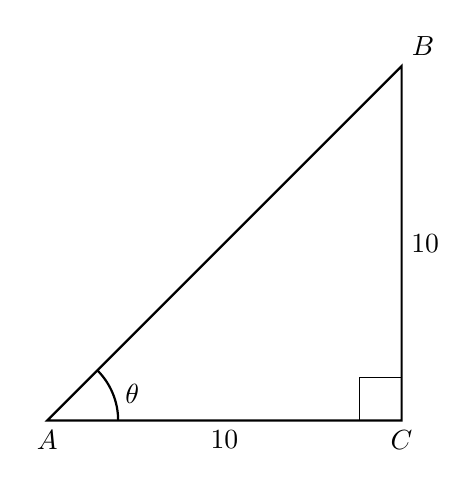
\begin{tikzpicture}[scale=0.9]
        \draw [thick](0,0)node[below]{$A$}--
        (5,0)node[below]{$C$}--
        (5,5)node[above right]{$B$}--cycle;
        \draw (5,0)++(-0.6,0)--++(0,0.6)--+(0.6,0);
        \node at (2.5,0)[below]{$10$};
        \node at (5,2.5)[right]{$10$};
        \draw [thick, -] (1,0) arc [start angle=0, end angle=45, radius=1];
        \node at (1.2,0.1)[above]{$\theta$};
      \end{tikzpicture}
    \end{flushright}
  \end{multicols} \vspace{1cm}

\item Given right triangle $\triangle ABC$ with base $AC=1$ and hypotenuse $AB=2$ as marked.\vspace{0.25cm}
\begin{enumerate}[itemsep=1.cm]
  \begin{multicols}{2}
    \item Find the altitude $BC=h$. \vspace{1cm}
    \item $\triangle ABC$ is reflected across $\overline{BC}$. Mark the lengths of the sides of its image $\triangle DBC$ 
    \item Write down the angle measure of $\angle A$.
\begin{flushright}
        \begin{tikzpicture}[scale=1]
        \draw [thick]
        (0,0)node[below]{$A$}--
        (3,0)node[below]{$C$}--
        (60:6)node[above]{$B$}--cycle;
        \draw (3,0)++(-0.5,0)--++(0,0.5)--+(0.5,0);
        \draw [dashed] (3,0)--(6,0)node[below]{$D$}--(60:6);
        \node at (1.5,0)[below]{$1$};
        \node at (62:3)[left]{$2$};
        \node at (3,2)[right]{$h$};
      \end{tikzpicture}
\end{flushright}
\end{multicols}
\item Write down the angle measure of $\angle ABC$.
\item Write down $\cos A$.
\item Write down $\sin A$.
\vspace{1cm}
\end{enumerate}
\vspace{1cm}

\newpage
\item In the diagram below, $\triangle ABC$ is inscribed in circle $O$. Show that $\overline{AB} \perp \overline{BC}$.
    \begin{flushright}
      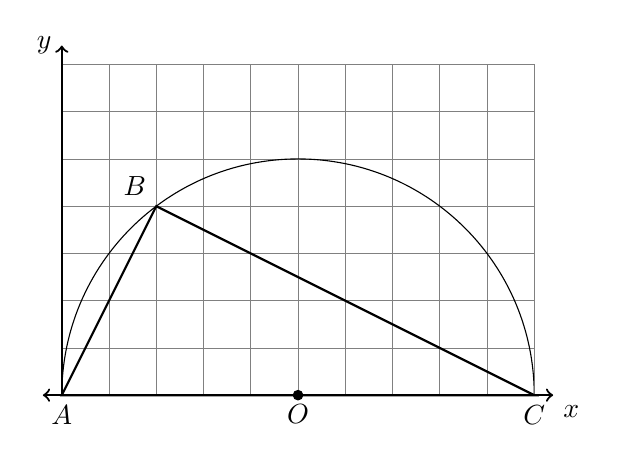
\begin{tikzpicture}[scale=0.6]
        \draw [help lines] (0,0) grid (10,7);
        \draw [thick, <->] (-0.4,0) -- (10.4,0) node [below right] {$x$};
        \draw [thick, ->] (0,0)--(0,7.4) node [left] {$y$};
        \draw [thick]
          (0,0)node[below]{$A$}--
          (2,4) node[above left]{$B$}--
          (10,0) node[below]{$C$}--cycle;
        \draw [fill] (5,0) circle [radius=0.1] node[below] {$O$};
        \clip (0,0) rectangle (10,6);
        \draw (5,0) circle [radius=5];
      \end{tikzpicture}
    \end{flushright} \vspace{1cm}

\item In the diagram below, $\triangle ABC$ has vertices with coordinates $A(1,2)$, $B(8,3)$ and $C(4, 6)$.
    \begin{center} %4 quadrant regents grid
      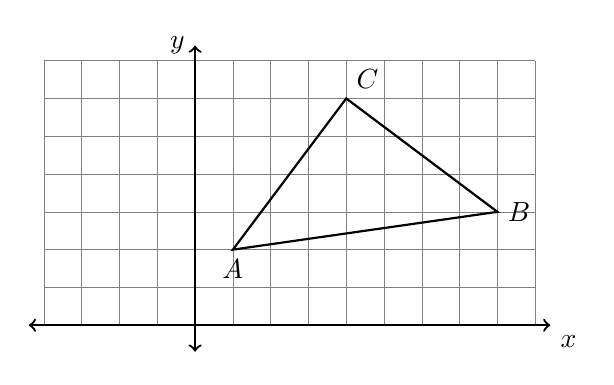
\begin{tikzpicture}[scale=.48]
        \draw [help lines] (-4,0) grid (9,7);
        \draw [thick, <->] (-4.4,0) -- (9.4,0) node [below right] {$x$};
        \draw [thick, <->] (0,-0.7)--(0,7.4) node [left] {$y$};
        \draw [thick]
          (1,2)node[below]{$A$}--
          (8,3) node[right]{$B$}--
          (4,6) node[above right]{$C$}--cycle;
        %\draw [fill] (-1,2) circle [radius=0.1] node[above left] {$A$};
        %draw [fill] (8, -4) circle [radius=0.1] node[below right] {$C$};
      \end{tikzpicture}
    \end{center}
    Find the length of each side of $\triangle ABC$, showing that it is isosceles and not equilateral.\\[0.5cm]
      \begin{tabular}{c|c|c}
        $AC=$ & $BC=$ & $AB=$ \\
        $\sqrt{(x_C-x_A)^2+(y_C-y_A)^2}$ & $\sqrt{(x_C-x_B)^2+(y_C-y_B)^2}$ & $ \sqrt{(x_B-x_A)^2+(y_B-y_A)^2}$ \\
        & & \\
        & & \\
      \end{tabular}

\end{enumerate}
\end{document}
  